\documentclass[11pt]{article}

\input{../../Latex_Common/skinnerr_latex_preamble_asen5417.tex}

%%
%% DOCUMENT START
%%

\begin{document}

\pagestyle{fancyplain}
\lhead{}
\chead{}
\rhead{}
\lfoot{\hrule ASEN 5417: Homework 8}
\cfoot{\hrule \thepage}
\rfoot{\hrule Ryan Skinner}

\noindent
{\Large Homework 8}
\hfill
{\large Ryan Skinner}
\\[0.5ex]
{\large ASEN 5417: Numerical Methods}
\hfill
{\large Due 2015/12/8}\\
\hrule
\vspace{6pt}

%%%%%%%%%%%%%%%%%%%%%%%%%%%%%%%%%%%%%%%%%%%%%%%%%
%%%%%%%%%%%%%%%%%%%%%%%%%%%%%%%%%%%%%%%%%%%%%%%%%
\section{Introduction} %%%%%%%%%%%%%%%%%%%%%%%%%%
%%%%%%%%%%%%%%%%%%%%%%%%%%%%%%%%%%%%%%%%%%%%%%%%%
%%%%%%%%%%%%%%%%%%%%%%%%%%%%%%%%%%%%%%%%%%%%%%%%%

Consider the linear convection-diffusion equation
\begin{equation}
\pp{T}{t} + v \pp{T}{y} = \alpha \pp{^2T}{y^2}
\;, \qquad
v = \sin(\pi y)
\;, \qquad
\alpha = \frac{1}{\text{Pr}\;\text{Re}}
\;,
\label{eq:conv-diff}
\end{equation}
subject to the initial conditions
\begin{equation}
\begin{aligned}
\text{(a)} && T(y,t=0) &= \cos(2 \pi y) \sin(\pi y) \\
\text{(b)} && T(y,t=0) &= \cos(2 \pi y)
\;,
\end{aligned}
\end{equation}
and parameters
\begin{equation}
\begin{aligned}
\text{Re} &= 1 &\quad &\text{(Reynolds number, molten glass)} \\
\text{Pr} &= 25 &\quad &\text{(Prandtl number, molten glass)} \\
\Delta t &= 0.001 &\quad &\text{(Time step)} \\
L_y &= 2 &\quad &\text{(Domain $y$-length)} \\
N &= 2^n + 1 &\quad &\text{(Number of $y$-points, where $n=5,6$)}
\;.
\end{aligned}
\end{equation}

\subsection{Problem 1}

Use the Fourier pseudo-spectral (FPS) method to numerically integrate \eqref{eq:conv-diff} with the given parameters. Use the Euler explicit method for time advancement. Higher resolution with $n=6$ will improve the accuracy of the method for the initial condition (a). Plot $T$ as a function of time $t$ at $t = \{0.2, 2, 5, 10\}$.

\subsection{Problem 2}

Use the FTCS Euler explicit method with second-order finite differences for the same computation, and compare results to the FPS method using the same mesh resolution.

%%%%%%%%%%%%%%%%%%%%%%%%%%%%%%%%%%%%%%%%%%%%%%%%%
%%%%%%%%%%%%%%%%%%%%%%%%%%%%%%%%%%%%%%%%%%%%%%%%%
\section{Methodology} %%%%%%%%%%%%%%%%%%%%%%%%%%%
%%%%%%%%%%%%%%%%%%%%%%%%%%%%%%%%%%%%%%%%%%%%%%%%%
%%%%%%%%%%%%%%%%%%%%%%%%%%%%%%%%%%%%%%%%%%%%%%%%%

\subsection{Problem 1}

We re-write \eqref{eq:conv-diff} as
\begin{equation}
\pp{T}{t} = \alpha \pp{^2T}{y^2} - v \pp{T}{y}
\;.
\end{equation}
The first and second spatial derivatives of $T$ are calculated by taking the Fourier transform of $T$, multiplying the Fourier coefficients by $i k_n$ and $-k_n^2$, respectively to take the first and second derivatives in Fourier space, and then taking the inverse Fourier transform to recover the first and second derivatives in physical space. With values of $\partial T / \partial t$ known at all grid points, values of $T$ at the next time step are calculated using the explicit Euler method,
\begin{equation}
T^{n+1} = T^n + \Delta t \pp{T}{t}
\;.
\end{equation}

\subsection{Problem 2}

To implement the FTCS explicit method, we approximate \eqref{eq:conv-diff} using forward-differences in time and central-differences in space as
\begin{equation}
\frac{T_i^{n+1} - T_i^n}{\Delta t}
+ v \frac{T_{i+1}^n - T_{i-1}^n}{2 \Delta y}
=
\alpha \frac{T_{i+1}^n - 2 T_i^n + T_{i-1}^n}{\Delta y^2}
\;,
\end{equation}
which can be solved for $T_i^{n+1}$ as
\begin{equation}
T_i^{n+1}
=
T_i^n +
\Delta t
\left(
\alpha \frac{T_{i+1}^n - 2 T_i^n + T_{i-1}^n}{\Delta y^2}
- v \frac{T_{i+1}^n - T_{i-1}^n}{2 \Delta y}
\right)
\;.
\end{equation}
This constitutes an explicit equation for $T^{n+1}$; we can advance in time without the need to solve any matrix equations. We enforce periodic boundary conditions by wrapping $T_{i-1}$ to $T_{N}$ when $i=1$ and vice versa.

%%%%%%%%%%%%%%%%%%%%%%%%%%%%%%%%%%%%%%%%%%%%%%%%%
%%%%%%%%%%%%%%%%%%%%%%%%%%%%%%%%%%%%%%%%%%%%%%%%%
\section{Results} %%%%%%%%%%%%%%%%%%%%%%%%%%%%%%%
%%%%%%%%%%%%%%%%%%%%%%%%%%%%%%%%%%%%%%%%%%%%%%%%%
%%%%%%%%%%%%%%%%%%%%%%%%%%%%%%%%%%%%%%%%%%%%%%%%%

Since most interesting behavior occurs for $t<4$, we neglect to display solutions for the later requested times of $t = \{5, 10\}$. Based on computations performed but not presented here, the trends observed during $t<4$ can be extrapolated in these cases.

\subsection{Problem 1}

Solutions to the linear convection-diffusion equation using the FPS method are shown in \figref{fig:Prob1}.

\begin{figure}[p!]
\begin{center}
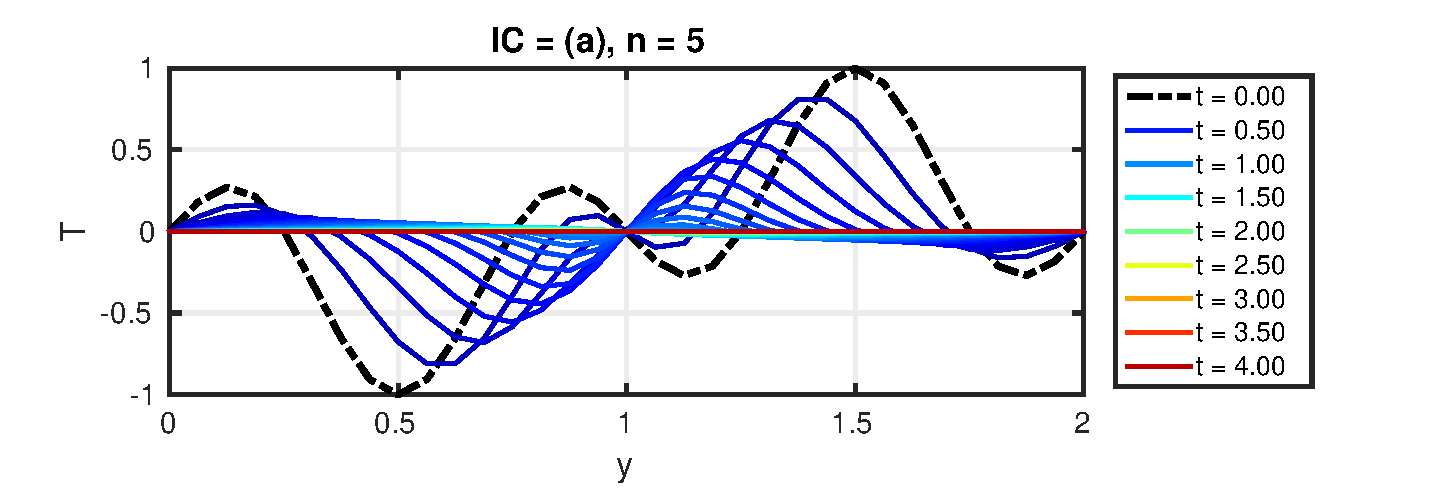
\includegraphics[width=0.85\textwidth]{Prob1_a5.eps} \\
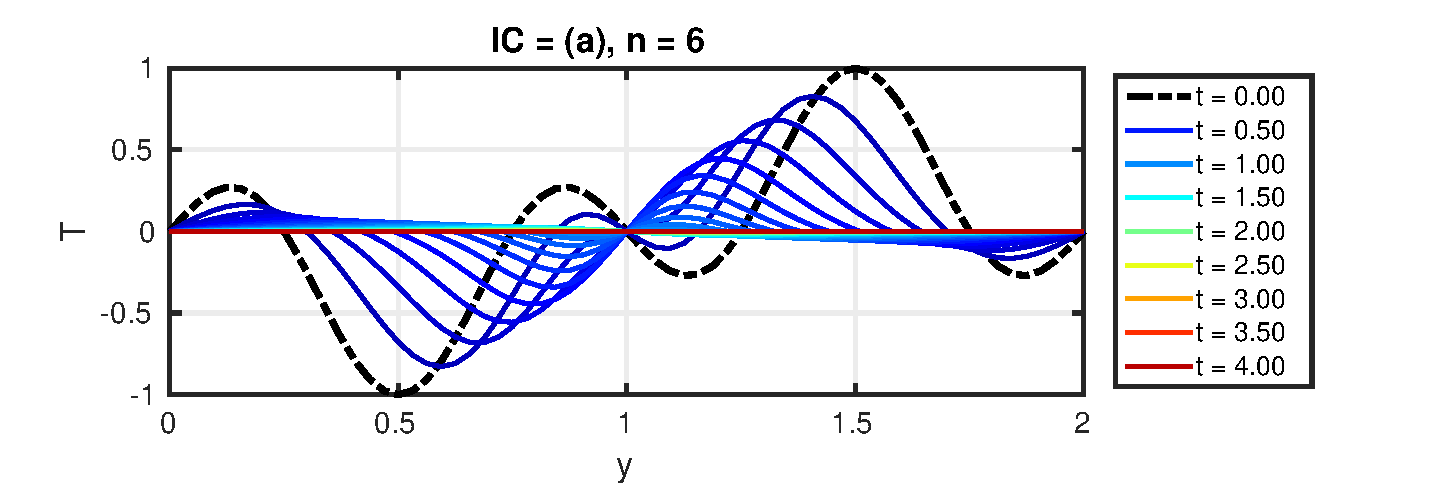
\includegraphics[width=0.85\textwidth]{Prob1_a6.eps} \\
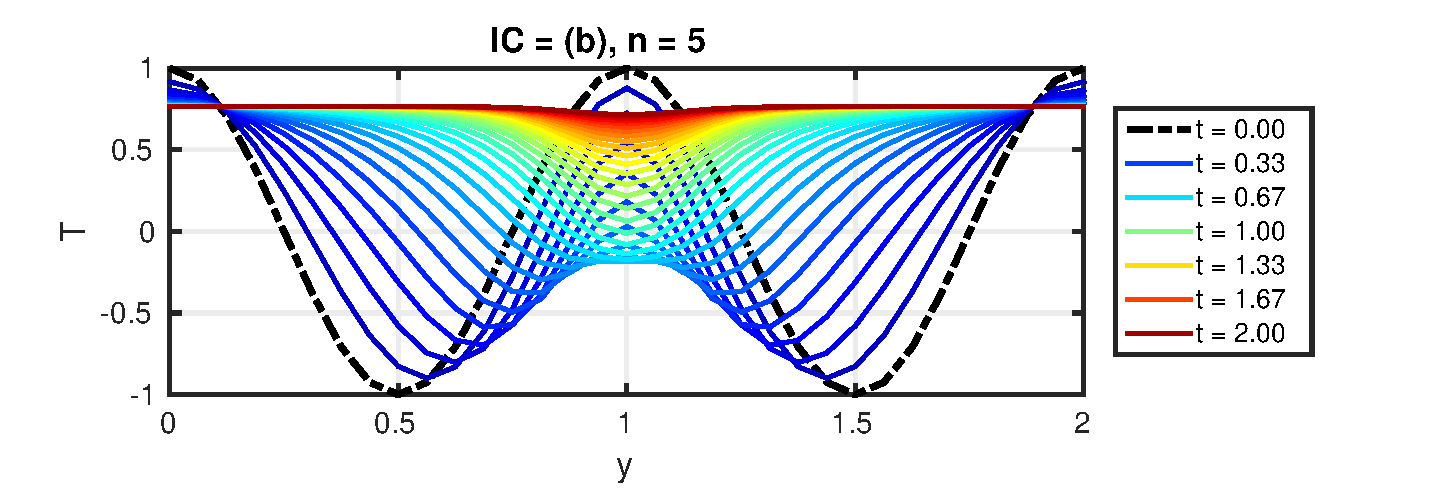
\includegraphics[width=0.85\textwidth]{Prob1_b5.eps} \\
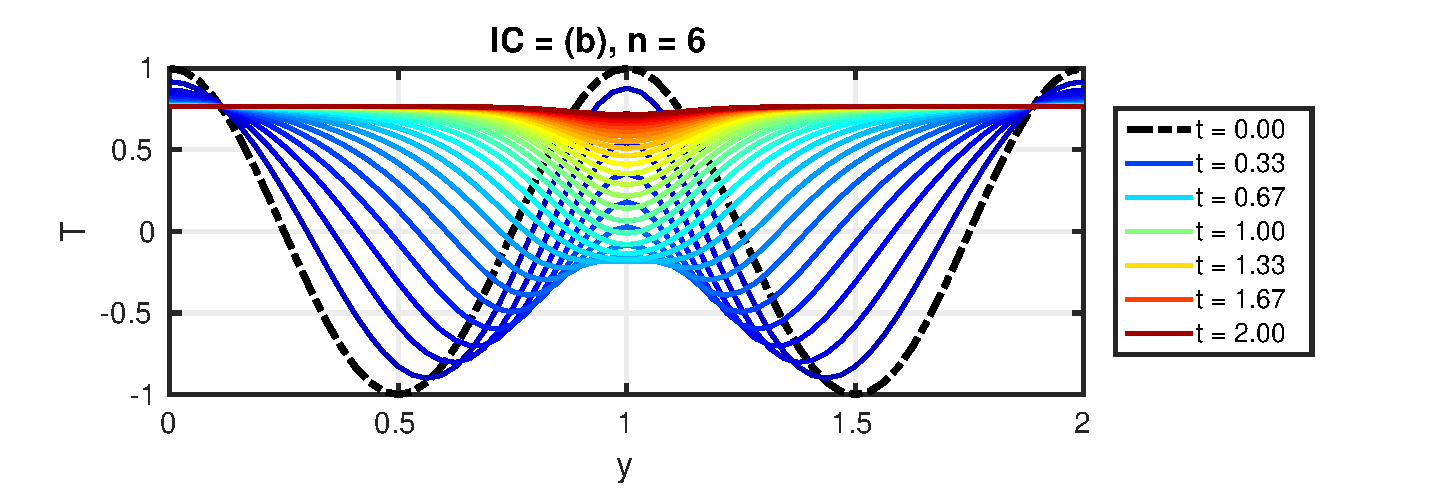
\includegraphics[width=0.85\textwidth]{Prob1_b6.eps}
\\[0.5cm]
\caption{Solutions to the linear convection-diffusion equation using the FPS method for different initial conditions and mesh resolution parameters. Most interesting behavior occurs when $t<4$. Trends can be extrapolated to future times $t=5, 10$, which are not shown. Initial condition displayed as black dot-dashed line (\dotdashrule).}
\label{fig:Prob1}
\end{center}
\end{figure}

\subsection{Problem 2}

Solutions using the FTCS method are compared to those from the FPS method in \figref{fig:Prob2_comparison}. The difference between the two methods, $T_\text{FPS} - T_\text{FTCS}$, at various time steps is shown in \figref{fig:Prob2_error}.

\begin{figure}[p!]
\begin{center}
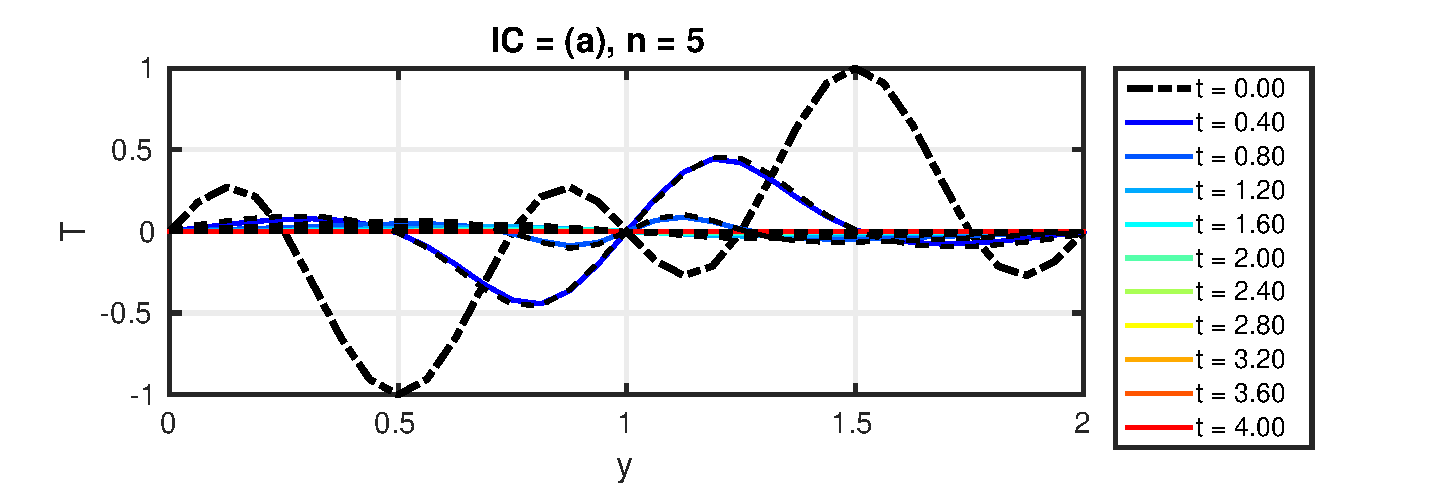
\includegraphics[width=0.85\textwidth]{Prob2_a5_comparison.eps} \\
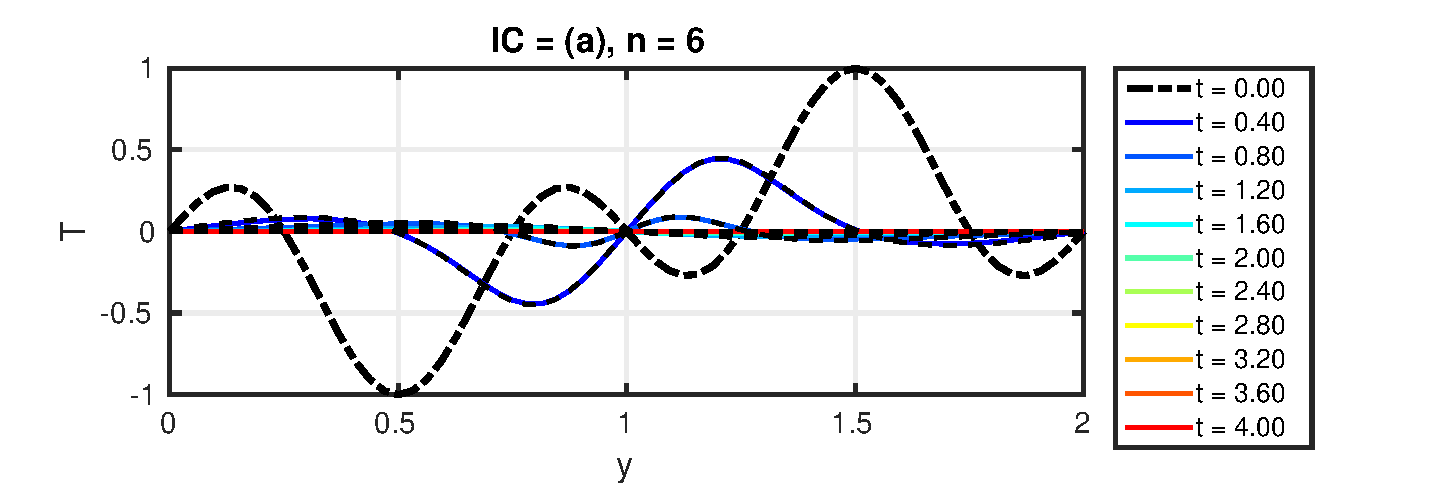
\includegraphics[width=0.85\textwidth]{Prob2_a6_comparison.eps} \\
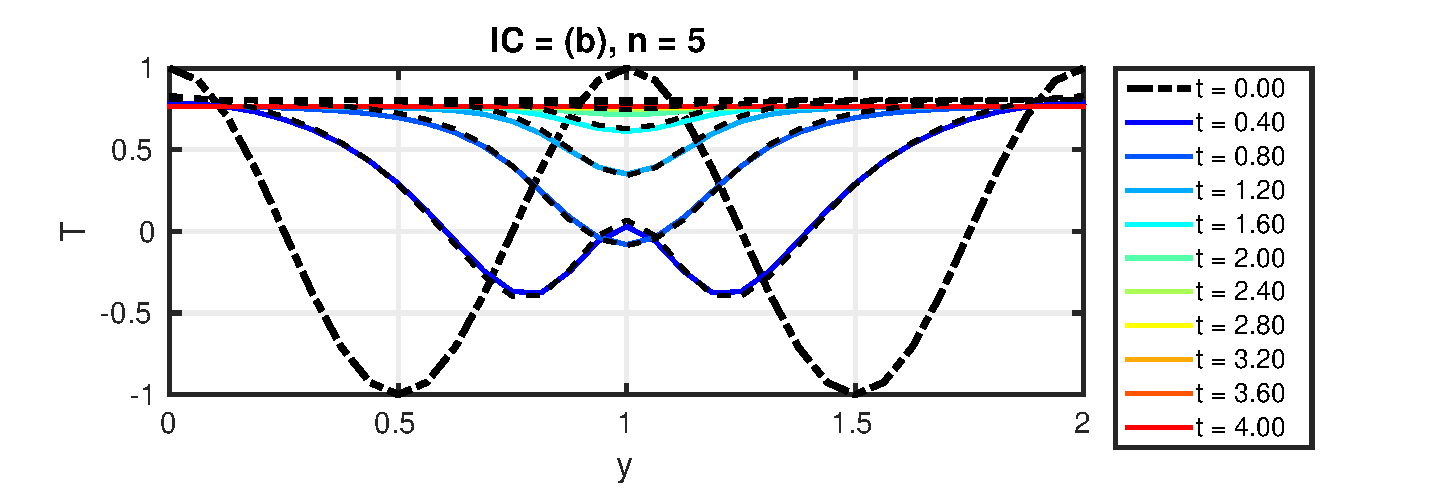
\includegraphics[width=0.85\textwidth]{Prob2_b5_comparison.eps} \\
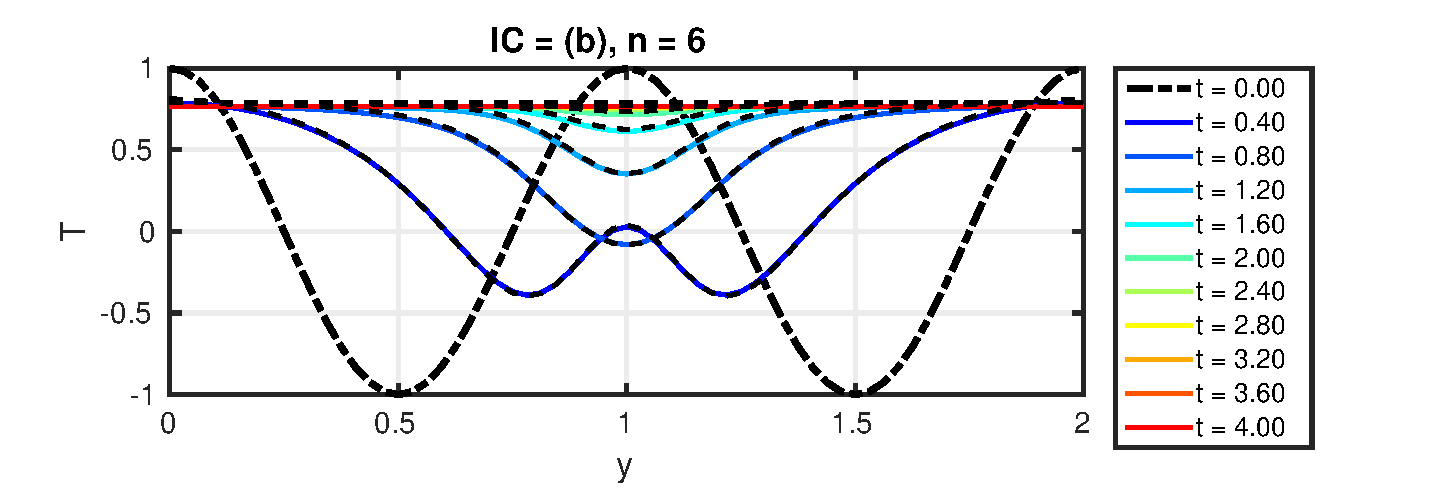
\includegraphics[width=0.85\textwidth]{Prob2_b6_comparison.eps}
\\[0.5cm]
\caption{Solution comparison between the FPS method (colored lines) and the FTCS method (\dashrule) for $t<4$. Initial condition displayed as black dot-dashed line (\dotdashrule). Agreement between the FPS and FTCS methods is decent. The limiting FPS value is $T \sim 0.765$ for both $n=\{5,6\}$, whereas the FTCS method's limiting values are $T \sim \{0.806, 0.788\}$ respectively. Further analysis is deferred to \figref{fig:Prob2_error}.}
\label{fig:Prob2_comparison}
\end{center}
\end{figure}

\begin{figure}[p!]
\begin{center}
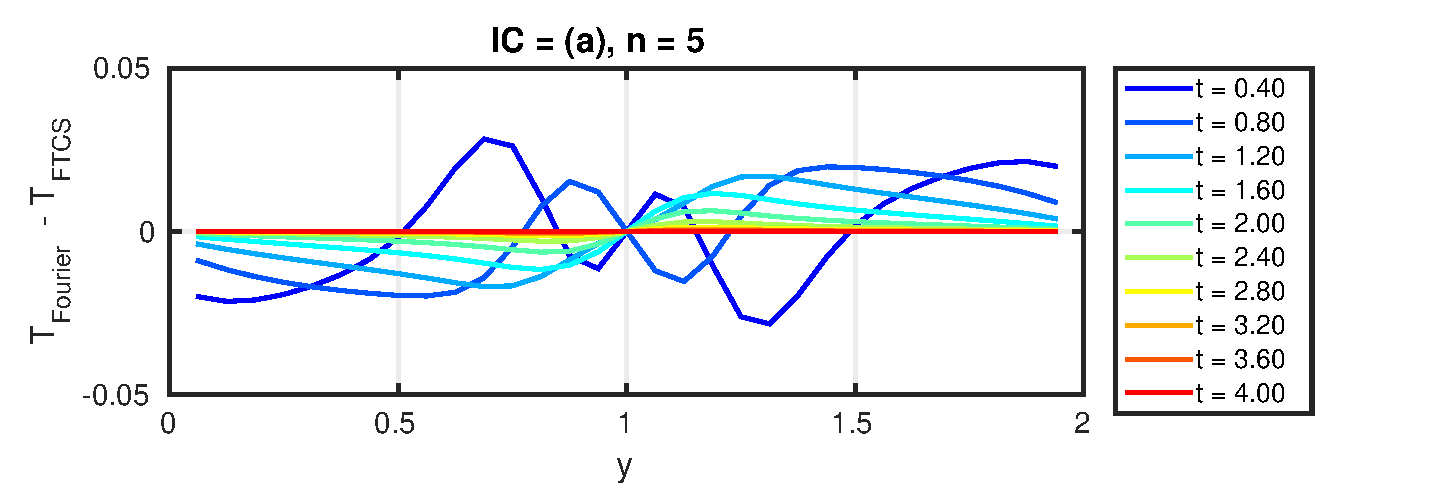
\includegraphics[width=0.85\textwidth]{Prob2_a5_error.eps} \\
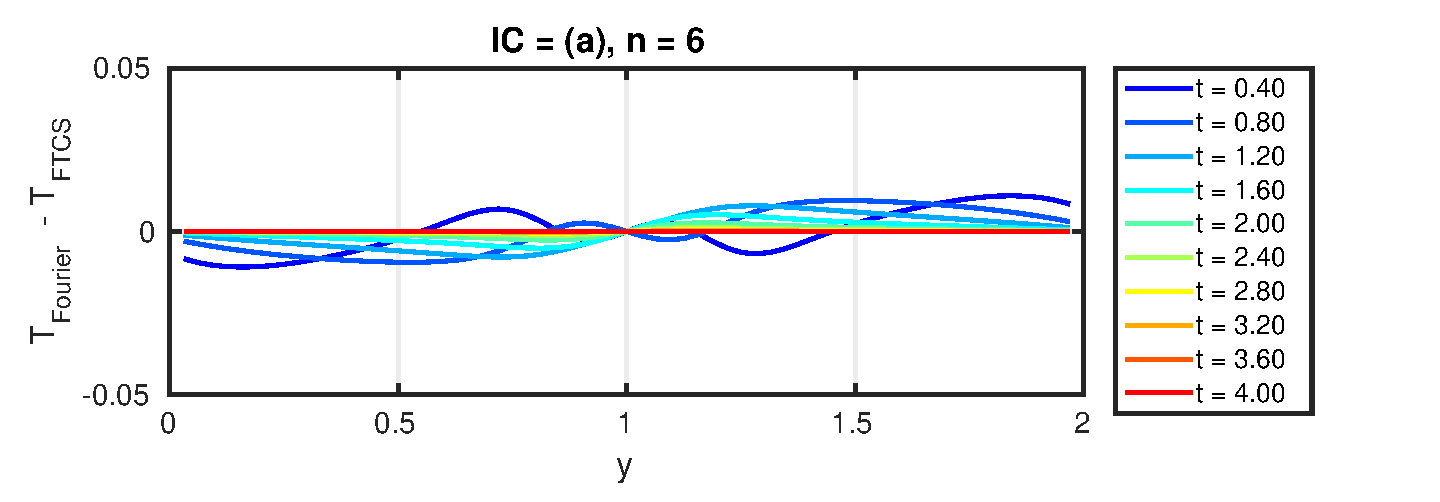
\includegraphics[width=0.85\textwidth]{Prob2_a6_error.eps} \\
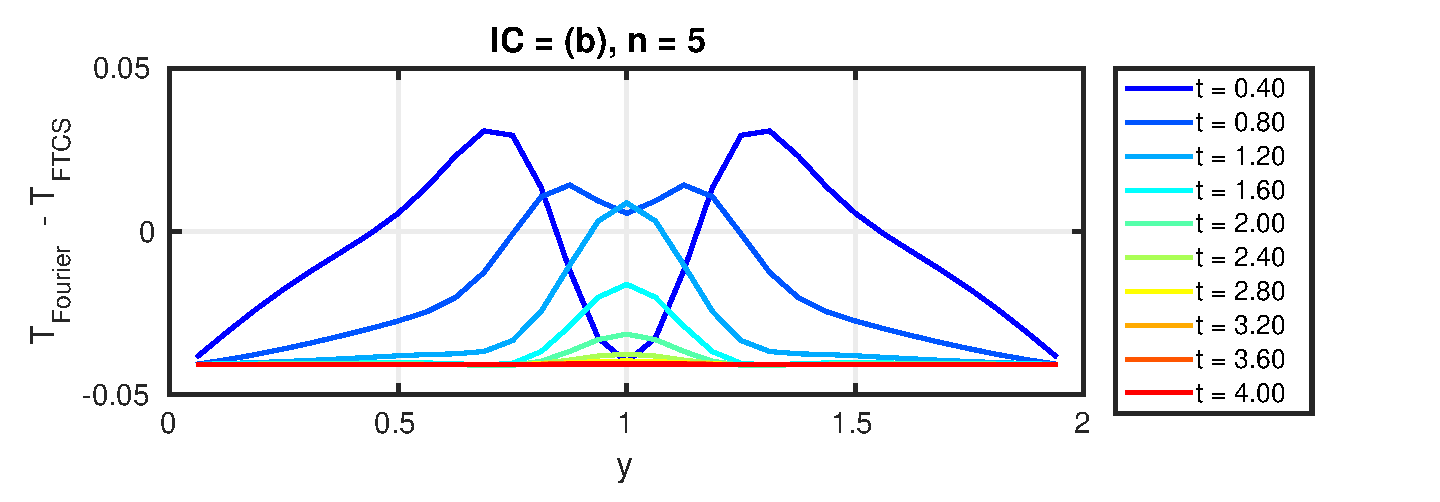
\includegraphics[width=0.85\textwidth]{Prob2_b5_error.eps} \\
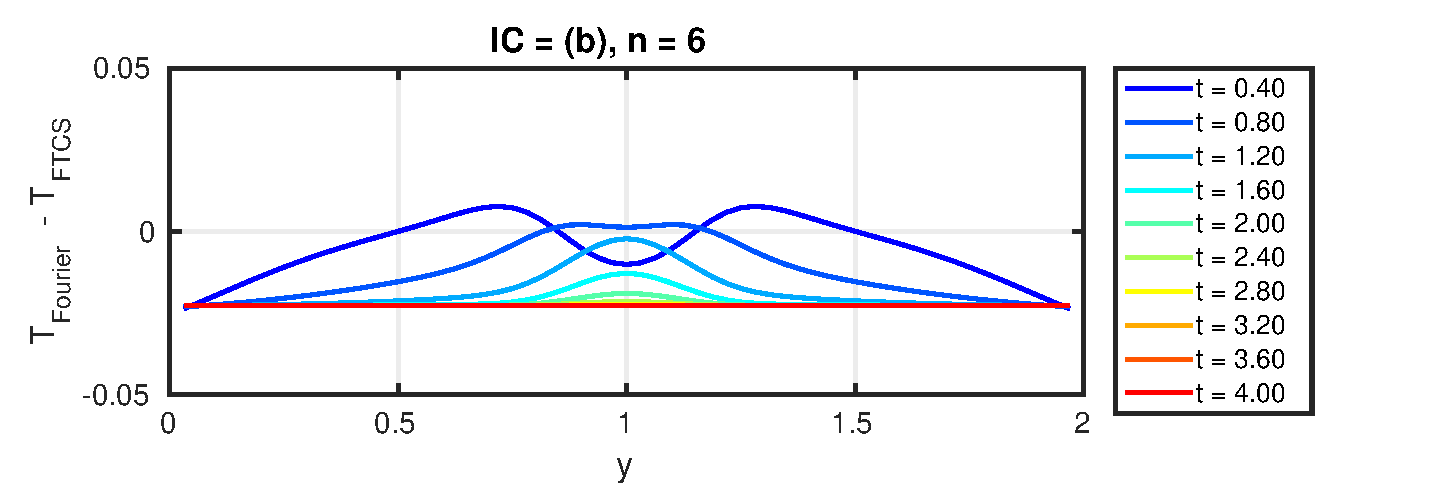
\includegraphics[width=0.85\textwidth]{Prob2_b6_error.eps}
\\[0.5cm]
\caption{Difference between the FPS and FTCS solutions at evenly-spaced discrete times $t<4$, omitting the initial condition. Different initial conditions and spatial resolutions produce different behavior.}
\label{fig:Prob2_error}
\end{center}
\end{figure}

%%%%%%%%%%%%%%%%%%%%%%%%%%%%%%%%%%%%%%%%%%%%%%%%%
%%%%%%%%%%%%%%%%%%%%%%%%%%%%%%%%%%%%%%%%%%%%%%%%%
\section{Discussion} %%%%%%%%%%%%%%%%%%%%%%%%%%%%
%%%%%%%%%%%%%%%%%%%%%%%%%%%%%%%%%%%%%%%%%%%%%%%%%
%%%%%%%%%%%%%%%%%%%%%%%%%%%%%%%%%%%%%%%%%%%%%%%%%

Both methods qualitatively predict the convection and diffusion behavior of both initial conditions at both mesh resolutions fairly well. In agreement with the given expression for convective velocity $v$, $T$ is convected toward $y=1$ at a rate sinusoidally dependent upon the distance to the center of the spatial domain. For initial condition (a), the initial condition sets $T=0$ at all points where $v=0$. Thus as positive and negative values of $T$ convect equally toward the domain center, diffusion smooths the equilibrium $T$ field to zero at all spatial locations. For initial condition (b), locations where $v=0$ correspond to locations where $T=1$. The negative values of $T$ convect toward the center rapidly and diffuse, resulting in an equilibrium value at all spatial points of $T \sim 0.765$.

Though the FPS and FTCS methods appear qualitatively similar in \figref{fig:Prob2_comparison}, the error plots in \figref{fig:Prob2_error} reveal some shortcomings of the latter. First, as the grid is refined in \figref{fig:Prob2_error}, it is no surprise that the point-wise discrepancies between methods decrease in magnitude. Furthermore, the FTCS method for initial condition (b) has difficulty capturing diffusion accurately. The equilibrium FPS value is $T \sim 0.765$ for both $n=\{5,6\}$ (likely grid-independent), whereas the FTCS method's limiting values are $T \sim \{0.806, 0.788\}$, respectively, and trend toward the equilibrium value of the FPS method with roughly $5\%$ and $3\%$ error. If we take the FPS solution as `truth,' which is not unreasonable for these periodic problems, the FTCS method suffers during the convection-dominated stage of the solution as well. Here, absolute point-wise errors can be as high as $0.04$ for $n=5$, which constitutes a $4\%$ error relative to the maximum initial $T$.

We conclude that the FPS method is superior to the FTCS method for period problems such as the linear convection-diffusion equation studied here, especially for low-$n$ grids.

%%%%%%%%%%%%%%%%%%%%%%%%%%%%%%%%%%%%%%%%%%%%%%%%%
%%%%%%%%%%%%%%%%%%%%%%%%%%%%%%%%%%%%%%%%%%%%%%%%%
\section{References} %%%%%%%%%%%%%%%%%%%%%%%%%%%%
%%%%%%%%%%%%%%%%%%%%%%%%%%%%%%%%%%%%%%%%%%%%%%%%%
%%%%%%%%%%%%%%%%%%%%%%%%%%%%%%%%%%%%%%%%%%%%%%%%%

No external references were used other than the course notes for this assignment.

%%%%%%%%%%%%%%%%%%%%%%%%%%%%%%%%%%%%%%%%%%%%%%%%%
%%%%%%%%%%%%%%%%%%%%%%%%%%%%%%%%%%%%%%%%%%%%%%%%%
\section*{Appendix: MATLAB Code} %%%%%%%%%%%%%%%%
%%%%%%%%%%%%%%%%%%%%%%%%%%%%%%%%%%%%%%%%%%%%%%%%%
%%%%%%%%%%%%%%%%%%%%%%%%%%%%%%%%%%%%%%%%%%%%%%%%%

The following code listings generate all figures presented in this homework assignment. The Fourier codes \lstinline|find_dfdn.m| and \lstinline|find_d2fdn2.m| are provided by Prof.\ Biringen.

\includecode{Problem_1.m}
\includecode{find_dfdn.m}
\includecode{find_d2fdn2.m}
\includecode{Problem_2.m}

%%
%% DOCUMENT END
%%
\end{document}
